\documentclass{article}
\usepackage[paper=a3paper, landscape, margin=0.5cm]{geometry}
\setlength\parskip{\bigskipamount}
\setlength\parindent{0pt}

\usepackage{tikz}
\usetikzlibrary{arrows}

\usepackage{longtable}

\usepackage{fontspec}
\usepackage[RTLdocument]{bidi}
\setmainfont[Mapping=tex-text, Script=Hebrew, Language=Hebrew]{Guttman Hatzvi}

\newcommand{\setsize}[1]{\fontsize{#1}{#1}\selectfont}

\usepackage{xcolor, graphicx}
\pagecolor{black}


\begin{document}

\begin{center}
\color{magenta!75!white}
\setsize{50}

~
\vfill

\resizebox{\linewidth}{!}{אהבה אינה יודעת מגדר}

\vfill

\resizebox{\linewidth}{!}{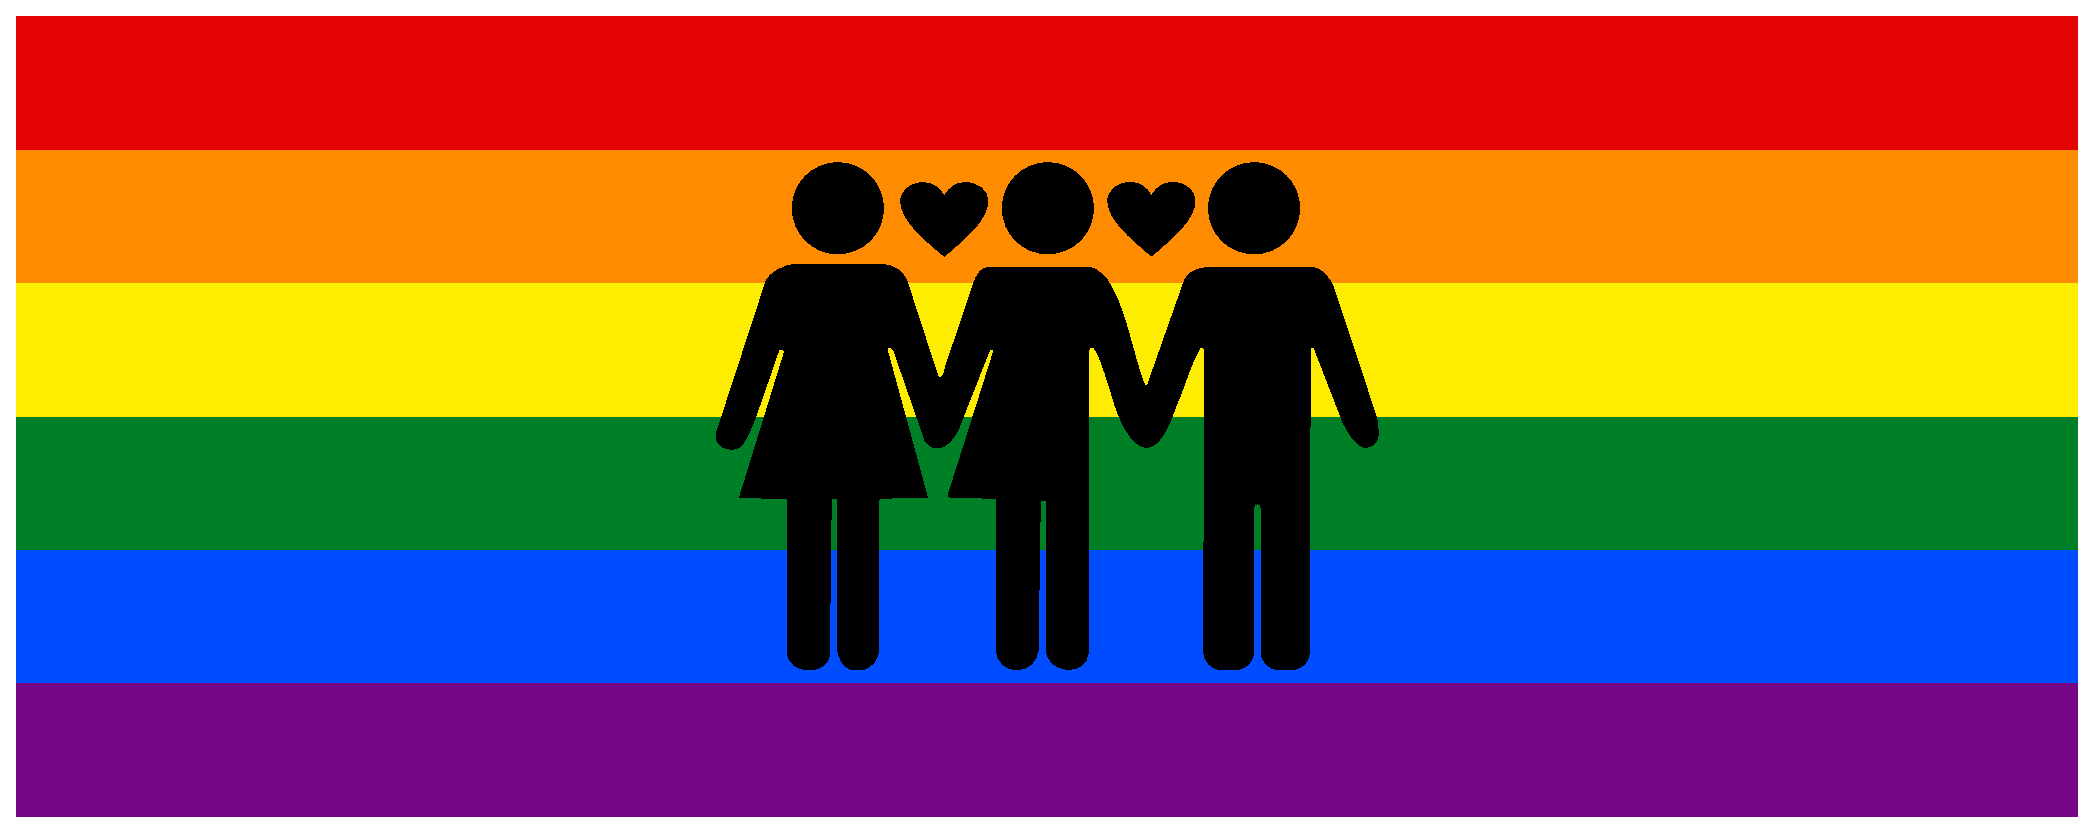
\includegraphics{polyamory.eps}} 

\vfill

\resizebox{\linewidth}{!}{היא גם לא יודעת לספור}

\vfill

~

\end{center}

\newpage

\begin{tikzpicture}
    \useasboundingbox [fill=magenta!75!white] (0,0) rectangle (\linewidth,0.5\paperheight);

	\node  at (0.5\linewidth,0.275\paperheight){
	\color{black}
	\setsize{110}
\RL{~\textbf{לא עלה תאנה ורוד!} \includegraphics[height=2ex]{figleaf.png}}};

\end{tikzpicture}

\vfill

\begin{center}
\setsize{60}
\color{magenta!75!white}

מתנגדת להוורדת {\fontspec{Alef}(pinkwashing)}
משטר ההפרדה הגזענית
של מדינת ישראל

\end{center}


%\resizebox{\linewidth}{!}{מתנגדת להוורדת ({\fontspec{Alef Bold}pinkwashing}) משטר}

%\resizebox{\linewidth}{!}{ההפרדה הגזענית של מדינת ישראל}}

\vfill

~
\end{document}

\newpage

~

\vfill

\fontsize{170}{170}
\addfontfeature{Color=FF00FFFF}

\begin{center}
	\vspace{-3cm}
	\noindent
		\hspace{-7cm}שחרור\\
		\hspace{-7cm}מגדרות\\
		\hspace{-7cm}המגדר
\end{center}

\vspace{-16.25cm}
\includegraphics[width=6.25cm]{cutter.png}

\vspace{-17.75cm}
~\hfill
\includegraphics[width=13cm]{gender.png}

\vfill

\begin{center}
\begin{tikzpicture}
	\begin{scope}[color=green]
	\def\wall{
		\foreach \x in {0,...,4}
			\filldraw (\x,0) rectangle (\x+0.9,2);
	}
	\def\tower{
		\filldraw (0.1,3.2) rectangle (0.9,3.3);
		\filldraw (-0.1,3.1)--(1.1,3.1)--(0.9,2.8)--(0.1,2.8)--cycle;
		\filldraw (0.1,2.7) rectangle (0.9,0);
	}


	\begin{scope}[xshift=0cm]
		\begin{scope}[xshift=0cm]\wall\end{scope}
	\end{scope}
	\begin{scope}[xshift=4.9cm]
		\tower
		\begin{scope}[xshift=1cm]\wall\end{scope}
		\begin{scope}[xshift=6cm]\wall\end{scope}
	\end{scope}
	\begin{scope}[xshift=15.8cm]
		\tower
		\begin{scope}[xshift=1cm]\wall\end{scope}
		\begin{scope}[xshift=6cm]\wall\end{scope}
	\end{scope}
	\begin{scope}[xshift=26.7cm]
		\tower
		\begin{scope}[xshift=1cm]\wall\end{scope}
		\begin{scope}[xshift=6cm]\wall\end{scope}
	\end{scope}
	\begin{scope}[xshift=37.6cm]
		\tower
		\filldraw (1,0) rectangle (1+0.9,2);
		\filldraw (2,0) rectangle (2+0.9,2);
	\end{scope}
	\filldraw (0,-0.1) rectangle (40.5,-0.3);
	\end{scope}
\end{tikzpicture}
\end{center}

\newpage

\fontsize{100}{100}
\normalfont
\addfontfeature{Color=FF00FF}

\begin{center}
	\textbf{אף אחד לא חופשי\\עד שלא כולם חופשיים}
\end{center}

\vfill

\vspace{2.5cm}
\setLR
\begin{longtable}{p{0.2\linewidth}p{0.6\linewidth}p{0.2\linewidth}}
%~\hfill
\includegraphics[height=9cm]{hand.png}
\hfill~
&
\begin{center}
	\vspace{-10.5cm}
	\RL{
		\fontsize{110}{110}
		\normalfont
		%\addfontfeature{Color=ff40b9}
		\addfontfeature{Color=00FF00}
		\textbf{ללא חומות\newline
		ללא מחסומים\newline
		ללא מכלאות}
		}
\end{center}
&
~\hfill
\hspace{0.4cm}\includegraphics[height=9cm]{paw.png}
\hfill~
%2
\end{longtable}
\setRL

\vfill

\fontsize{90}{90}
\normalfont
\begin{center}
	\vspace{-6cm}
	{\textbf{\addfontfeature{Color=00FF00} ללא גבולות \addfontfeature{Color=FF00FFFF} של מין, מגדר, נטייה מינית, מוצא, מעמד, זן}}
\end{center}

